%%%%%%%%%%%%%%%%%%%%%%%%%%%%%%%%%%%%%%%%%
% Journal Article
% LaTeX Template
% Version 1.3 (9/9/13)
%
% This template has been downloaded from:
% http://www.LaTeXTemplates.com
%
% Original author:
% Frits Wenneker (http://www.howtotex.com)
%
% License:
% CC BY-NC-SA 3.0 (http://creativecommons.org/licenses/by-nc-sa/3.0/)
%
%%%%%%%%%%%%%%%%%%%%%%%%%%%%%%%%%%%%%%%%%

%----------------------------------------------------------------------------------------
%  PACKAGES AND OTHER DOCUMENT CONFIGURATIONS
%----------------------------------------------------------------------------------------

\documentclass[twoside]{article}\usepackage[]{graphicx}\usepackage[]{color}
%% maxwidth is the original width if it is less than linewidth
%% otherwise use linewidth (to make sure the graphics do not exceed the margin)
\makeatletter
\def\maxwidth{ %
  \ifdim\Gin@nat@width>\linewidth
    \linewidth
  \else%
    \Gin@nat@width
  \fi
}
\makeatother

\definecolor{fgcolor}{rgb}{0.345, 0.345, 0.345}
\newcommand{\hlnum}[1]{\textcolor[rgb]{0.686,0.059,0.569}{#1}}%
\newcommand{\hlstr}[1]{\textcolor[rgb]{0.192,0.494,0.8}{#1}}%
\newcommand{\hlcom}[1]{\textcolor[rgb]{0.678,0.584,0.686}{\textit{#1}}}%
\newcommand{\hlopt}[1]{\textcolor[rgb]{0,0,0}{#1}}%
\newcommand{\hlstd}[1]{\textcolor[rgb]{0.345,0.345,0.345}{#1}}%
\newcommand{\hlkwa}[1]{\textcolor[rgb]{0.161,0.373,0.58}{\textbf{#1}}}%
\newcommand{\hlkwb}[1]{\textcolor[rgb]{0.69,0.353,0.396}{#1}}%
\newcommand{\hlkwc}[1]{\textcolor[rgb]{0.333,0.667,0.333}{#1}}%
\newcommand{\hlkwd}[1]{\textcolor[rgb]{0.737,0.353,0.396}{\textbf{#1}}}%

\usepackage{framed}
\makeatletter
\newenvironment{kframe}{%
 \def\at@end@of@kframe{}%
 \ifinner\ifhmode%
  \def\at@end@of@kframe{\end{minipage}}%
  \begin{minipage}{\columnwidth}%
 \fi\fi%
 \def\FrameCommand##1{\hskip\@totalleftmargin \hskip-\fboxsep
 \colorbox{shadecolor}{##1}\hskip-\fboxsep
     % There is no \\@totalrightmargin, so:
     \hskip-\linewidth \hskip-\@totalleftmargin \hskip\columnwidth}%
 \MakeFramed {\advance\hsize-\width
   \@totalleftmargin\z@ \linewidth\hsize
   \@setminipage}}%
 {\par\unskip\endMakeFramed%
 \at@end@of@kframe}
\makeatother

\definecolor{shadecolor}{rgb}{.97, .97, .97}
\definecolor{messagecolor}{rgb}{0, 0, 0}
\definecolor{warningcolor}{rgb}{1, 0, 1}
\definecolor{errorcolor}{rgb}{1, 0, 0}
\newenvironment{knitrout}{}{} % an empty environment to be redefined in TeX

\usepackage{alltt}

\usepackage{lipsum} % Package to generate dummy text throughout this template

\usepackage[sc]{mathpazo} % Use the Palatino font
\usepackage[T1]{fontenc} % Use 8-bit encoding that has 256 glyphs
\linespread{1.05} % Line spacing - Palatino needs more space between lines
\usepackage{microtype} % Slightly tweak font spacing for aesthetics

\usepackage[hmarginratio=1:1,top=32mm,columnsep=20pt]{geometry} % Document margins
\usepackage{multicol} % Used for the two-column layout of the document
\usepackage[hang, small,labelfont=bf,up,textfont=it,up]{caption} % Custom captions under/above floats in tables or figures
\usepackage{booktabs} % Horizontal rules in tables
\usepackage{float} % Required for tables and figures in the multi-column environment - they need to be placed in specific locations with the [H] (e.g. \begin{table}[H])
\usepackage{hyperref} % For hyperlinks in the PDF

\usepackage{lettrine} % The lettrine is the first enlarged letter at the beginning of the text
\usepackage{paralist} % Used for the compactitem environment which makes bullet points with less space between them

\usepackage{abstract} % Allows abstract customization
\renewcommand{\abstractnamefont}{\normalfont\bfseries} % Set the "Abstract" text to bold
\renewcommand{\abstracttextfont}{\normalfont\small\itshape} % Set the abstract itself to small italic text

\usepackage{titlesec} % Allows customization of titles
\renewcommand\thesection{\Roman{section}} % Roman numerals for the sections
\renewcommand\thesubsection{\Roman{subsection}} % Roman numerals for subsections
\titleformat{\section}[block]{\large\scshape\centering}{\thesection.}{1em}{} % Change the look of the section titles
\titleformat{\subsection}[block]{\large}{\thesubsection.}{1em}{} % Change the look of the section titles

\usepackage{fancyhdr} % Headers and footers
\pagestyle{fancy} % All pages have headers and footers
\fancyhead{} % Blank out the default header
\fancyfoot{} % Blank out the default footer
\fancyhead[C]{Running title $\bullet$ November 2012 $\bullet$ Vol. XXI, No. 1} % Custom header text
\fancyfoot[RO,LE]{\thepage} % Custom footer text
\bibliographystyle{plain}

%%%-------------------------------------------------%%%
%%% Preferences for Knitr %%%
%%%-------------------------------------------------%%%


%%%-------------------------------------------------%%%
%%% Sub document global preferences for Knitr %%%
%%%-------------------------------------------------%%%










%----------------------------------------------------------------------------------------
%  TITLE SECTION
%----------------------------------------------------------------------------------------

\title{\vspace{-15mm}\fontsize{24pt}{10pt}\selectfont\textbf{Article Title}} % Article title

\author{
\large
\textsc{John Smith}\thanks{A thank you or further information}\\[2mm] % Your name
\normalsize University of California \\ % Your institution
\normalsize \href{mailto:john@smith.com}{john@smith.com} % Your email address
\vspace{-5mm}
}
\date{}

%----------------------------------------------------------------------------------------
\IfFileExists{upquote.sty}{\usepackage{upquote}}{}

\begin{document}

\maketitle % Insert title

\thispagestyle{fancy} % All pages have headers and footers

%----------------------------------------------------------------------------------------
%	ABSTRACT
%----------------------------------------------------------------------------------------

%%%-------------------------------------------------%%%
%%% Include abstract %%%
%%%-------------------------------------------------%%%


%%%-------------------------------------------------%%%
%%% Sub document abstract %%%
%%%-------------------------------------------------%%%

\begin{abstract}

% Remove the lipsum and fill in your abstract text here
\lipsum[1]

\end{abstract}




%----------------------------------------------------------------------------------------
%	ARTICLE CONTENTS
%----------------------------------------------------------------------------------------

\begin{multicols}{2} % Two-column layout throughout the main article text

%%%-------------------------------------------------%%%
%%% Include introduction %%%
%%%-------------------------------------------------%%%


%%%-------------------------------------------------%%%
%%% Sub document introduction %%%
%%%-------------------------------------------------%%%

\section{Introduction}

% Remove the lipsum and the list example and fill in your introduction text here

%\capital{T} his is just an introduction text snippet to show how drop caps look in this document.
\lipsum[1]
\cite{renwick_chemical_2002}

\begin{itemize}
  \item One
    \begin{itemize}
      \item One One
        \begin{itemize}
          \item One One One
        \end{itemize}
    \end{itemize}
  \item Two
  \item Three
\end{itemize}

\lipsum[1-2]


%%%-------------------------------------------------%%%
%%% Include data and methods %%%
%%%-------------------------------------------------%%%


%%%-------------------------------------------------%%%
%%% Sub document for data and methods %%%
%%%-------------------------------------------------%%%

\section{Data And Methods}

% Remove the lipsum and example table fill in your material and methods text here

\lipsum[1] 



%%%-------------------------------------------------%%%
%%% Include results %%%
%%%-------------------------------------------------%%%


%%%-------------------------------------------------%%%
%%% Sub document results %%%
%%%-------------------------------------------------%%%

\section{Results}

% Remove the lipsum and the example plots and tables to fill in your abstract text here

\subsection{Subheading}

\lipsum[1-2]

\begin{knitrout}
\definecolor{shadecolor}{rgb}{0.969, 0.969, 0.969}\color{fgcolor}
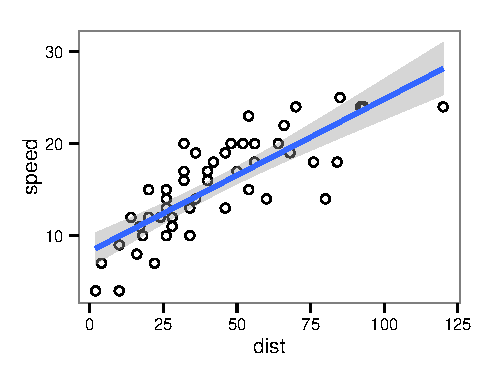
\includegraphics[width=\maxwidth]{figure/test_plot} 

\end{knitrout}


\lipsum 

\begin{equation}
   \sqrt[3]{1-y^2}
\end{equation}

\begin{knitrout}
\definecolor{shadecolor}{rgb}{0.969, 0.969, 0.969}\color{fgcolor}
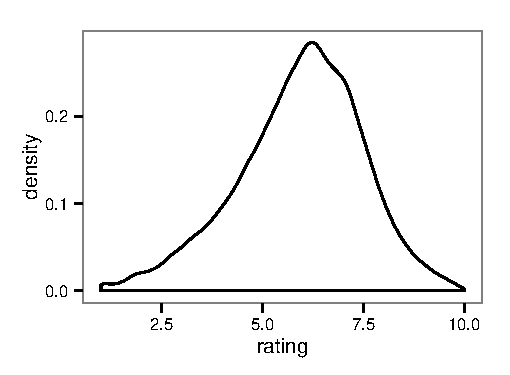
\includegraphics[width=\maxwidth]{figure/test_plot_two1} 

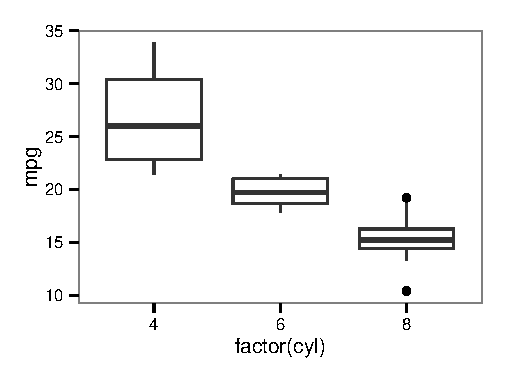
\includegraphics[width=\maxwidth]{figure/test_plot_two2} 

\end{knitrout}


\lipsum[1-5]



%%%-------------------------------------------------%%%
%%% Include discussion %%%
%%%-------------------------------------------------%%%


%%%-------------------------------------------------%%%
%%% Sub document for discussion %%%
%%%-------------------------------------------------%%%

\section{Discussion}

% Remove the lipsum and fill in your discussion text here
\lipsum[1-4]


%%%-------------------------------------------------%%%
%%% Include acknowledgements %%%
%%%-------------------------------------------------%%%


%%%-------------------------------------------------%%%
%%% Sub document for acknowledgement %%%
%%%-------------------------------------------------%%%

\section{Acknowledgements}

% Remove the lipsum and fill in your acknowledgements here
\lipsum[4-5]


%%%-------------------------------------------------%%%
%%% Include the bibliography %%%
%%%-------------------------------------------------%%%


\end{multicols}

\bibliography{bibliography/bib} 

%%%-------------------------------------------------%%%
%%% Include the appendix %%%
%%%-------------------------------------------------%%%


%%%-------------------------------------------------%%%
%%% Sub document for appendix %%%
%%%-------------------------------------------------%%%

\section{Appendix}




\end{document}
